\documentclass[aspectratio=43]{beamer}
\usepackage[utf8]{inputenc}

%%%%%%%%%%%%%%%%%%%%%%%% THEME
\usetheme{material}
\useLightTheme
\usePrimaryPurple
\useAccentTeal

\usepackage{macros} % must come after theme

\title{\q Tools}
\keywords{\qk}

\begin{document}

\begin{frame}
	\titlepage
\end{frame}


\begin{frame}{Table of contents}
	\begin{card}
		\tableofcontents
	\end{card}
\end{frame}

% What is the state of quantum software tools (find others)
% Python and Pip
% Jupyter notebooks (anaconda or lighter installation)
% IBM's qiskit
% Terra and aqua and other: https://medium.com/qiskit/qiskit-and-its-fundamental-elements-bcd7ead80492
% Tutorial on how to install qiskit
% Mention the community (slack, medium, maybe VsCode extension)
% Example code
% References and additional sources
% https://github.com/Qiskit/qiskit-tutorial

\section{Introduction}
\begin{frame}{Introduction}
    \begin{card}
    This week is all about getting to know the \textbf{tools} at our disposal. Some previous knowledge is required of the Python programming language, but other than that we will mention what matters the most about the tools in this course. Deeper and wider knowledge of them will arise with use!
    \end{card}
\pagenumber
\end{frame}


\section{Python}
\begin{frame}{Python}
    \begin{center}
	    
\includegraphics[width=0.5\textwidth]{python.png}
	\end{center}
    \begin{card}
        \href{https://www.python.org/}{Python} is a high-level scripting language that is widely used for prototyping due to its simplicity and abstractions. Most importantly, it has a huge community that builds and shares tools and frameworks that are easily used by Python users. Most of these \textbf{packages} are available at \href{https://pypi.org/}{PyPi} and can be installed easily through \mintinline{bash}{pip install PACKAGE_NAME}. 
    \end{card}
\pagenumber
\end{frame}

\section{Jupyter}
\begin{frame}{Jupyter}
    \begin{center}
	    
\includegraphics[width=0.2\textwidth]{jupyter}
	\end{center}
	\begin{cardTiny}
	    \href{http://jupyter.org/}{Project Jupyter} has produced an amazing tool, the Jupyter Notebooks: a web-based environment that can be used to write code as if it were a book, using markdown, executing code block by block, and viewing the output next to the code that produced it. This makes it easy to document, understand and share code.\\
	    We will be using these notebooks for most of the practical exercises.
	\end{cardTiny}
\pagenumber
\end{frame}

\begin{frame}{Installing Jupyter Notebooks}
    \begin{center}
	    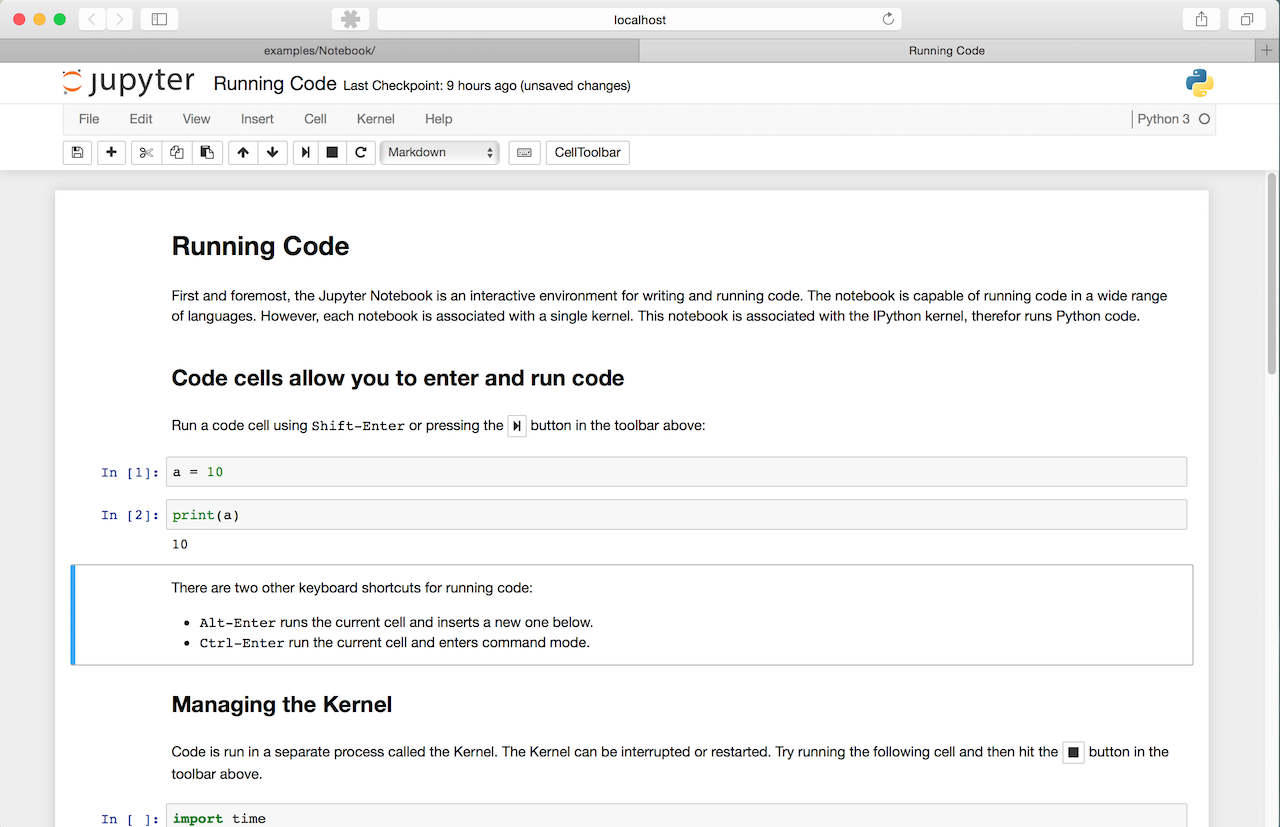
\includegraphics[width=0.8\textwidth]{jupyter_notebook}
	\end{center}
    \begin{cardTiny}
        \small{
        There are two options for installing Jupyter Notebooks in your computer, both properly described \href{http://jupyter.org/install.html}{here}. After that, head to a console and do \mintinline{bash}{jupyter notebook}. 
        }
    \end{cardTiny}
\pagenumber
\end{frame}

\section{Google Colaboratory}
\begin{frame}{Google Colaboratory}
    \begin{center}
	    
\includegraphics[width=0.3\textwidth]{colab}
    \end{center}
    \begin{cardTiny}
        Although it is still bellow critical mass (for now), there is an online version of Jupyter Notebooks that allows for collaborative and real-time edition of your notebooks (much like Google Docs): \href{https://colab.research.google.com/}{Google Colaboratory}!\\
        Even if it is not directly used in this course, you may find it useful to work with others and, at times, to use Jupyter Notebooks in computers without a local installation of Jupyter Notebooks.
    \end{cardTiny}
\pagenumber
\end{frame}


\section{Binder}
\begin{frame}{Binder}
    \begin{center}
	    
\includegraphics[width=0.7\textwidth]{mybinder}
    \end{center}
    \begin{cardTiny}
        Much like Colaboratory, Binder is a fantastic tool to interact with Jupyter Notebooks online and without any previous setup. This may come in useful in the future. However it is best suited for Notebooks hosted in GitHub, which is not a problem in \href{\githubRepo}{this course}.\\
        Binder is available at \href{https://mybinder.org/}{mybinder.org}!
    \end{cardTiny}
\pagenumber
\end{frame}


\section{\qk}
\begin{frame}{\qk}
    \begin{center}
	    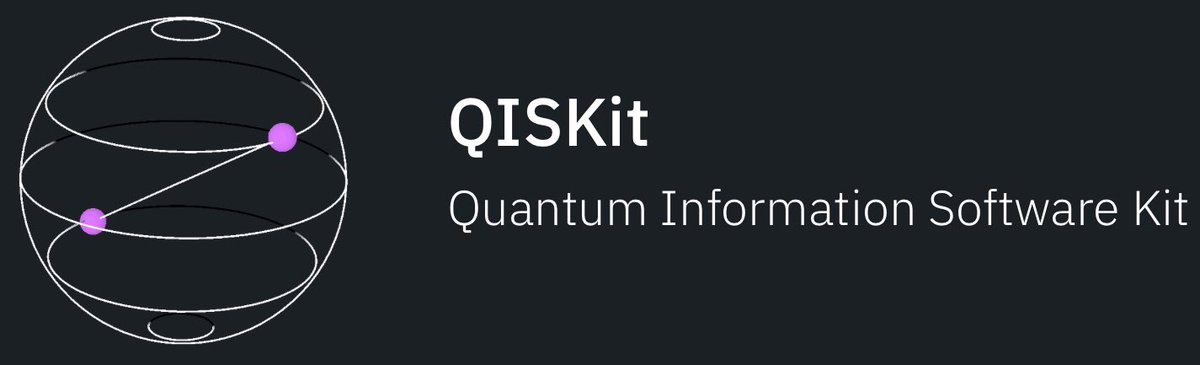
\includegraphics[width=0.8\textwidth]{qiskit}
    \end{center}
    \begin{cardTiny}
    Quoting, \qk is `an open-source quantum computing framework for leveraging today's quantum processors and conducting research'. It can be used through a python interface (our focus) and it is, no doubt, \textbf{the most important tool of this course}. (You read it like biscuit, but with a Q!)
    \end{cardTiny}
\pagenumber
\end{frame}


\begin{frame}{The \qk framework}
    \begin{center}
	    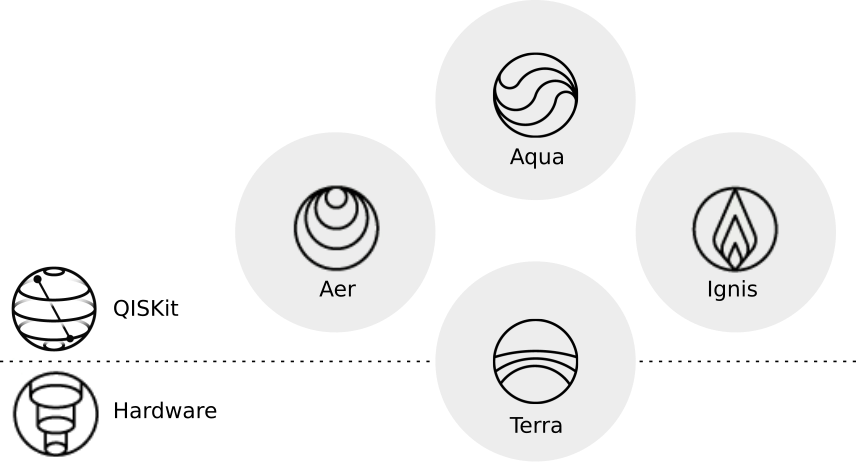
\includegraphics[width=0.65\textwidth]{qiskit_elements}
    \end{center}
    \begin{cardTiny}
        \small{
        The \qk framework is subdivided into four tools:
        \footnotesize{
            \begin{itemize}
                \itemsep0em 
                \item \qk Terra (\mintinline{bash}{pip install qiskit})
                \item \qk Ignis (part of qiskit package)
                \item \qk Aer (part of qiskit package)
                \item \qk Aqua  (\mintinline{bash}{pip install qiskit-aqua})
            \end{itemize}
        }
        }
    \end{cardTiny}
\pagenumber
\end{frame}


\begin{frame}{The \qk framework}
    \begin{cardTiny}
        \qk can be seen as a \textbf{Full Stack \q Framework}. It allows developers and researchers to both get 'their hands dirty` on low-level quantum gates (Terra) and also to work with all minutiae abstracted, as if it were a classical program (Aqua). 
    \end{cardTiny}
    \begin{cardTiny}
        We will mainly focus on \qk Terra. The following four \textit{fundamental slides} are based on \href{https://medium.com/qiskit/qiskit-and-its-fundamental-elements-bcd7ead80492}{this post} and provide the base understanding of each of these elements.
    \end{cardTiny}
    \begin{cardTiny}
        \small{\textbf{Installation Tip:}
        If \mintinline{bash}{pip install} fails, try \mintinline{bash}{pip3 install}. To change this behaviour on Linux, visit \href{https://askubuntu.com/a/321000}{this post}.
        }
    \end{cardTiny}
\pagenumber
\end{frame}


\subsection{\qk Terra}
\begin{frameImg}{qiskit_elements}
    \begin{card}[\qk Terra]
        `Terra, the \textit{earth} element, is the foundation on which the rest of the software lies. Terra provides a bedrock for composing quantum programs at the level of circuits and pulses, to optimize them for the constraints of a particular device, and to manage the execution of batches of experiments on remote-access devices. Terra defines the interfaces for a desirable end-user experience, as well as the efficient handling of layers of optimization, pulse scheduling and backend communication.'
    \end{card}
\pagenumber
\end{frameImg}

\subsection{\qk Aqua}
\begin{frameImg}{qiskit_elements}
    \begin{card}[\qk Aqua]
    `Aqua, the \textit{water} element, is the element of life. To make quantum computing live up to its expectations, we need to find real-world applications. Aqua is where algorithms for NISQ (Noisy Intermediate-Scale Quantum) computers are built. These algorithms can be used to build applications for quantum computing. Aqua is accessible to domain experts in chemistry, optimization or AI, who want to explore the benefits of using quantum computers as accelerators for specific computational tasks, without needing to worry about how to translate the problem into the language of quantum machines.'
    \end{card}
\pagenumber
\end{frameImg}

\subsection{\qk Ignis}
\begin{frameImg}{qiskit_elements}
    \begin{card}[\qk Ignis]
    `Ignis, the \textit{fire} element, is dedicated to fighting noise and errors and to forging a new path. This includes better characterization of errors, improving gates, and computing in the presence of noise. Ignis is meant for those who want to design quantum error correction codes, or who wish to study ways to characterize errors through methods such as tomography, or even to find a better way for using gates by exploring dynamical decoupling and optimal control. While we have already released parts of this element as part of libraries in Terra, an official stand-alone release will come soon.'
    \end{card}
\pagenumber
\end{frameImg}

\subsection{\qk Aer}
\begin{frameImg}{qiskit_elements}
    \begin{card}[\qk Aer]
        \small{`Aer, the \textit{air} element, permeates all Qiskit elements. To really speed up development of quantum computers we need better simulators, emulators and debuggers. At IBM Q, we have built high-quality, high-performance simulators and continue to improve their scalability and features. Aer will help us understand the limits of classical processors by demonstrating to what extent they can mimic quantum computation. Furthermore, we can use Aer to verify that current and near-future quantum computers function correctly. This can be done by stretching the limits of simulation to accommodate 50+ qubits with reasonably high depth, and by simulating the effects of realistic noise on the computation.'}
    \end{card}
\pagenumber
\end{frameImg}

\begin{frameImg}{qiskit_elements}
    \begin{card}[\qk Wrap-up]
    Each piece fits into the puzzle, and although you may end up working on high-level quantum code, in this course we will walk through all the low-level bases that will shed some more light into the \q beauty!\\
    Many new and potentially unknown terms were used in the definitions of these fundamental elements of \qk, in time some will become clearer and you will begin to see real implementation of these tools in your work. So don't worry if you feel lost, it is just to give you a glimpse of the \qw!
    \end{card}
\pagenumber
\end{frameImg}

\subsection{Community and VSCode extension}
\begin{frame}
    \begin{card}[Community]
        \qk brings along a growing community, you can interact with it through \href{https://qiskit.slack.com/}{Slack}, \href{https://github.com/Qiskit}{GitHub}, \href{https://medium.com/qiskit}{Medium}, \href{https://www.facebook.com/qiskit/}{Facebook} and more!
    \end{card}
    \begin{card}[VSCode extension]
        \href{https://code.visualstudio.com/}{VSCode} is an open-source code editor that is both light and extremely versatile, being extremely customisable to the code you need to write. \href{https://medium.com/qiskit/qiskit-vscode-extension-a-new-tool-to-enhance-your-quantum-programming-experience-951cc8c1954b}{Recently}, a new extension for \qk has been created which eases the whole process of developing for \qk. Check it on \href{https://github.com/Qiskit/qiskit-vscode}{GitHub}, as it may prove useful for this course and also for your future work.
    \end{card}
\pagenumber
\end{frame}

\section{\ibmqe}
\begin{frame}{\ibmqe}
\begin{card}
    Finally, on the list of main tools for this course, \ibmqe. This is a manifestation of all the more sidereal nature of \qk into the palpable world. \ibmq represents IBM's efforts of making \qc have an impact on industry and science.\\
    \ibmqe means IBM's \q Computers are accessible to the every day developer. To us, this means writing some quantum circuits and executing, not only in a simulation environment, but on one of the real \q Computers that IBM has. All you have to do is \href{https://quantumexperience.ng.bluemix.net/qx/signup}{create an account} and you are ready to \href{https://quantumexperience.ng.bluemix.net/qx/editor}{design and execute your circuits}!
\end{card}
\pagenumber
\end{frame}


\section{Exercises}
\begin{frame}{Exercises}
    For this week, there are some boring tasks:
    \begin{itemize}
        \item Install Python (and pip)
        \item Install Jupyter
        \item Install \qk
        \item Create an account on \ibmqe
    \end{itemize}
    As well as some interesting tasks:
    \begin{itemize}
        \item Checkout the community for \qk
        \item Do this week's exercises (local setup of IBMQ account)
    \end{itemize}
\pagenumber
\end{frame}

\section{Where to learn more?}
\begin{frame}{Where to learn more?}
\begin{card}
    \begin{itemize}
        \item \href{https://medium.com/qiskit/qiskit-and-its-fundamental-elements-bcd7ead80492}{Qiskit and its Fundamental Elements}
        \item \href{https://arxiv.org/abs/1801.00862}{Quantum Computing in the NISQ era and beyond, John Preskill}
        \item \href{https://docs.python.org/3/tutorial/}{Python tutorial} (plenty other tutorials out there)
        \item \href{https://www.datacamp.com/community/tutorials/tutorial-jupyter-notebook}{Jupyter tutorial}
    \end{itemize}
\end{card}
\end{frame}
\end{document}
